\documentclass[]{article}
\usepackage[hidelinks]{hyperref}
\usepackage{graphicx, amsmath, listings, amssymb, commath}
\usepackage[utf8]{inputenc}
\lstdefinestyle{mystyle}{
	showtabs=false, 
	tabsize=2
}

\lstdefinestyle{mystyle}{
	showtabs=false, 
	tabsize=2
}
\lstset{style=mystyle}
\usepackage[utf8]{inputenc}

\title{Rešitev 2. projektne naloge MM}
\author{Aljaž Verlič, Lina Lumborovska, Blažka Blatnik, Luka Tavčer \\
	Mentor: Damir Franetič}
\date{5. junij, 2017}

\begin{document}

\maketitle
\renewcommand{\abstractname}{Uvod}
%\begin{abstract}

%\end{abstract}

\textbf{\LARGE{Presek dveh implicitno danih ploskev}} \\\\\\\\
Vsebina:
\begin{enumerate}
	\item Opis naloge
	\item Delovanje metode
	\item Potrebni pogoj in Jacobijeva matrika
	\item Implementacija, testiranje in primere
	\item Analiza povpre\v{c}no \v{s}tevilo korakov Newtonove metode
	\item Koda
	\item Delitev dela v skupini
	\item Reference
\end{enumerate} 
\newpage

\section{Opis naloge}
	V $\mathbb{R}^3$ imamo podani dve poljubni implicitno podani ploskvi, opisanimi z enačbama $f_{1}(x)$ = $C_{1}$ in\\ $f_{2}(x)$ = $C_{2}$, presek pa je množica rešitev tega nelinearnega sistema enačb.\\
	Naša naloga je poiskati krivuljo $K$, ki predstavlja presek teh dveh ploskev. \\ \\
	Nalogo bomo rešili na 4 načine z uporabo metod za numerično reševanje diferencialnih enačb. Uporabili bomo:
	\begin{itemize}  
		\item Eulerjevo/Runge-Kutta s fiksno dolžino koraka
		\item Eulerjevo/Runge-Kutta z adaptivno dolžino koraka
	\end{itemize}

\section{Delovanje metode}
	nek text spredi še....\\
	\newline
	Opazimo, da je samo Eulerjeva metoda "blizu" pravilni rešitvi, ampak ni vredu.
	\begin{center}
		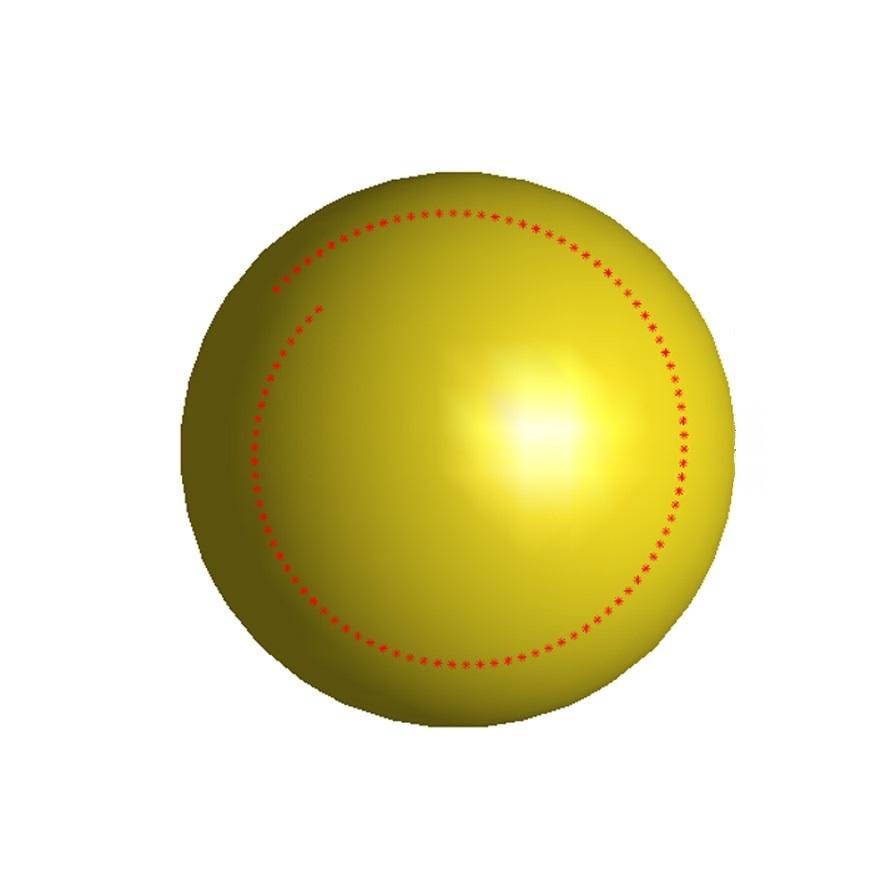
\includegraphics[scale=0.30]{eul1}
	\end{center}
	Napake se seštevajo in so na večjem intervalu bolj opazne.\\
	\begin{center}
		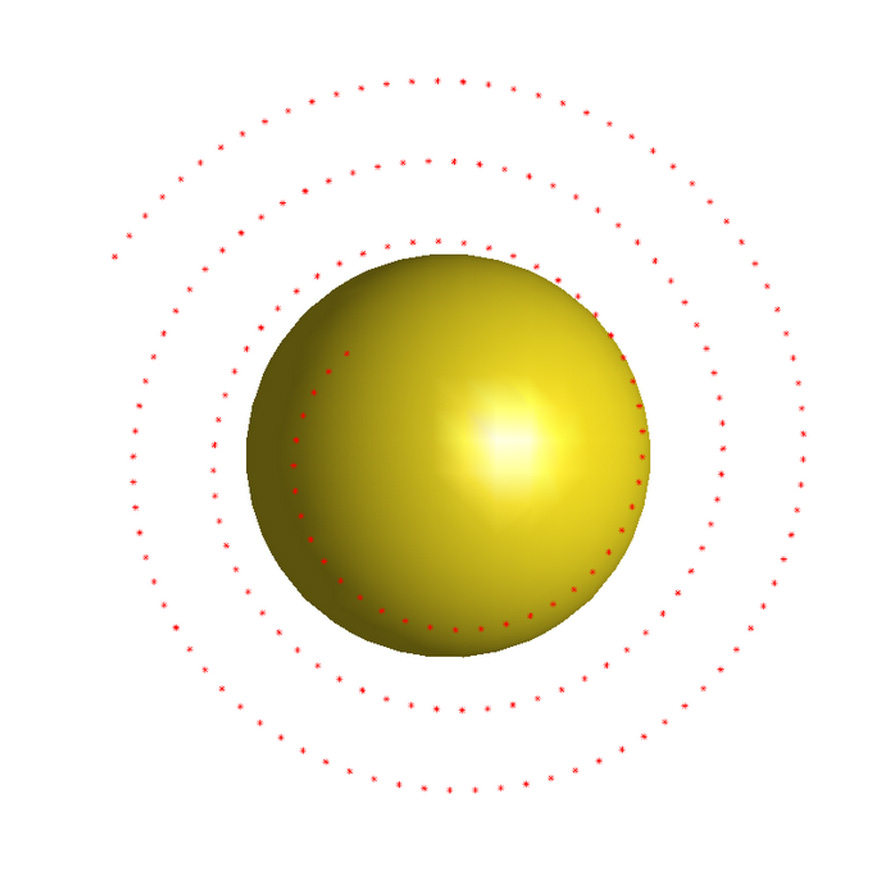
\includegraphics[scale=0.30]{eul2}
	\end{center}
	Ko za popravljanje napake uporabimo Newtonovo metodo, dobimo pravilno "krivuljo".\\
	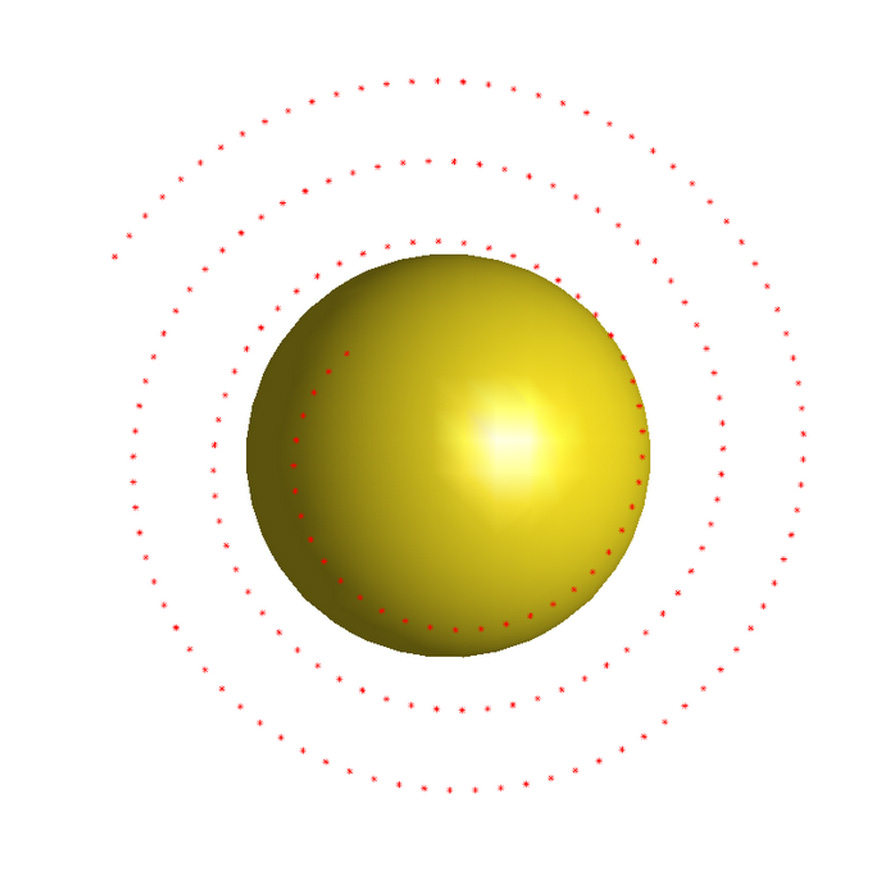
\includegraphics[scale=0.2]{eul2}
	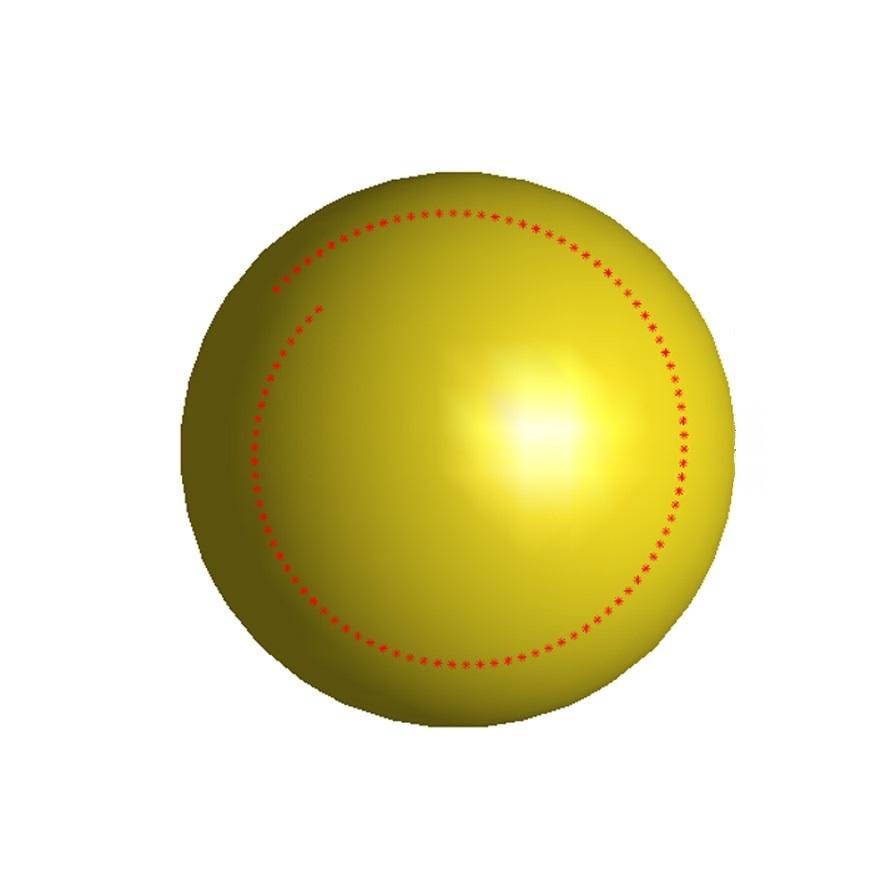
\includegraphics[scale=0.2]{eul1}
	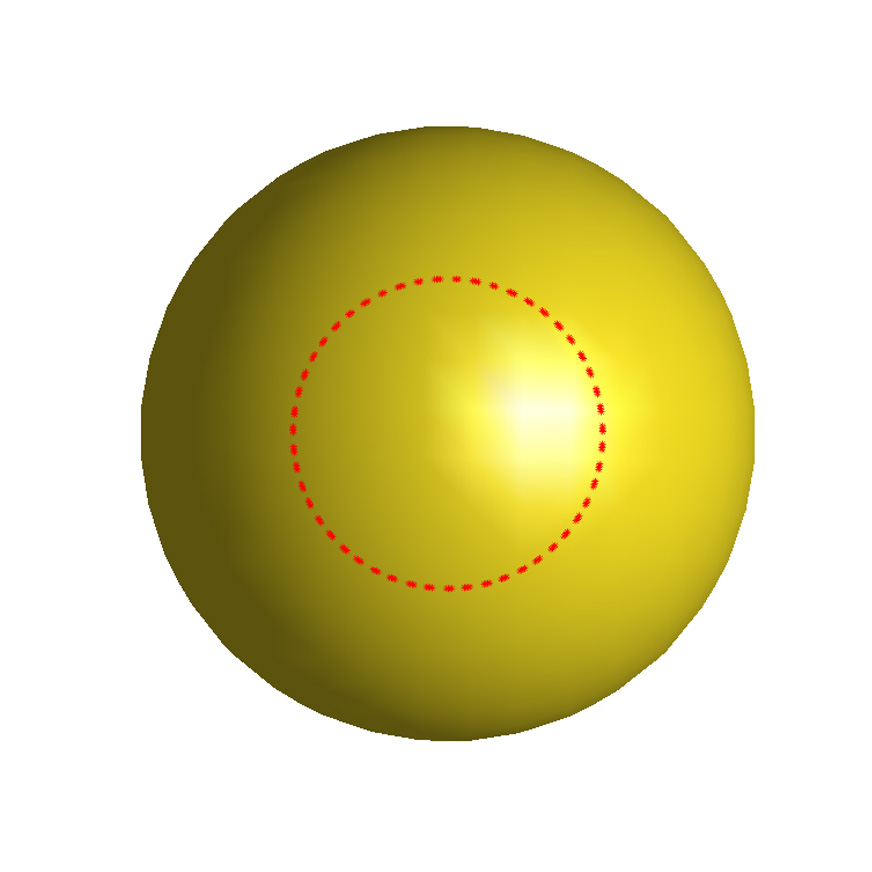
\includegraphics[scale=0.2]{eul3_newt}
	
\section{Potrebni pogoj in Jacobijeva matrika}
	Potreben pogoj za delovanje metod je, da sta funkciji $f_{1}$ in $f_{2}$ parcialno odvedljivi in da ima Jacobijeva matrika parcialnih odvodov poln rang 2. Za uspešno delovanje Newtonove metode moramo poiskati Jacobijevo matriko leve strani sistema nelinearnih enačb.

	\begin{center}
		JG = $\begin{bmatrix}
		grad(f_{1}) \\
		grad(f_{2}) \\
		\hspace{1mm}grad(\vec{v} \cdot \vec{x}) \\
		\end{bmatrix}$
		oziroma
		JG = $\begin{bmatrix}
		grad(f_{1}) \\
		grad(f_{2}) \\
		\hspace{1mm}grad(\vec{v}\hspace{0.5mm}^\intercal) \\
		\end{bmatrix}$
	\end{center}
	%[x, k] = newton(G, JG, x0, tol, maxit) poisce priblizek 
	%x za resitev enacbe F(x) = 0 z Newtonovo metodo.
	%(k je stevilo korakov, ki jih metoda porabi.)
	%G... funkcija
	%JG... Jacobijeva matrika G
	%x0... zacetni priblizek
	%tol... zahtevana natancnost
	%maxit... najvecje stevilo iteracij
	\begin{lstlisting}[language=Octave]
		function [x, k] = newton(G, JG, x0, tol, maxit)
			for k = 1:maxit
				%Izvedemo en korak Newtonove metode...
				x = x0 - feval(JG, x0)\feval(G, x0);
				
				if(norm(x - x0) < tol)	% Je metoda ze konvergirala?
					break;
				end
				x0 = x;
			endfor
			% Izpis opozorila, ce zadnji priblizek ni znotraj tolerance.
			if(k == maxit)
				disp("Warning: The method did not converge after maxit iterations.")
			end
		endfunction
	\end{lstlisting} \ \\

	%\includegraphics[scale=0.5]{sim_10x}

		
\section{Implementacija, testiranje in primere}
	Delovanje našega programa lahko preverimo s programom, ki smo ga napisali v Octave-u. Kot vhodne parametre mu podamo obe implicitno podani funkciji $f_{1}$, $f_{2}$, $C1$, $C2$, $grad(f_{1})$, $grad(f_{2})$. Določimo tudi začetni približek $x_{0}$, začetno dolžino koraka in pa parameter, ki določa metodo delovanja (Euler/Runge-Kutta).\\
	Program poženemo na različnih primerih in štejemo povprečno dolžino koraka ter število porabljenih korakov.\\\\
	Primer 1:
	\begin{itemize} 
		\item $f_{1}(x,y,z)$ = $x^2 + y^2 + z^2$ = 4
		\item $f_{2}(x,y,z)$ = $3x + 2y + z$ = 1	
	\end{itemize}
	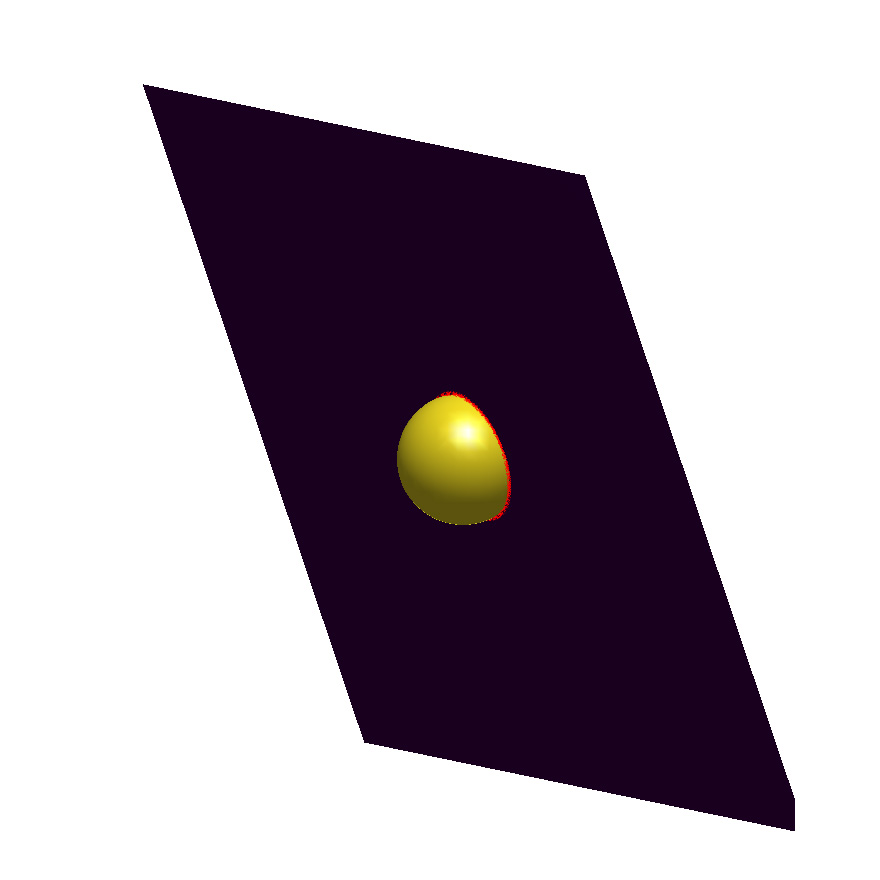
\includegraphics[scale=0.3]{primer1_1}
	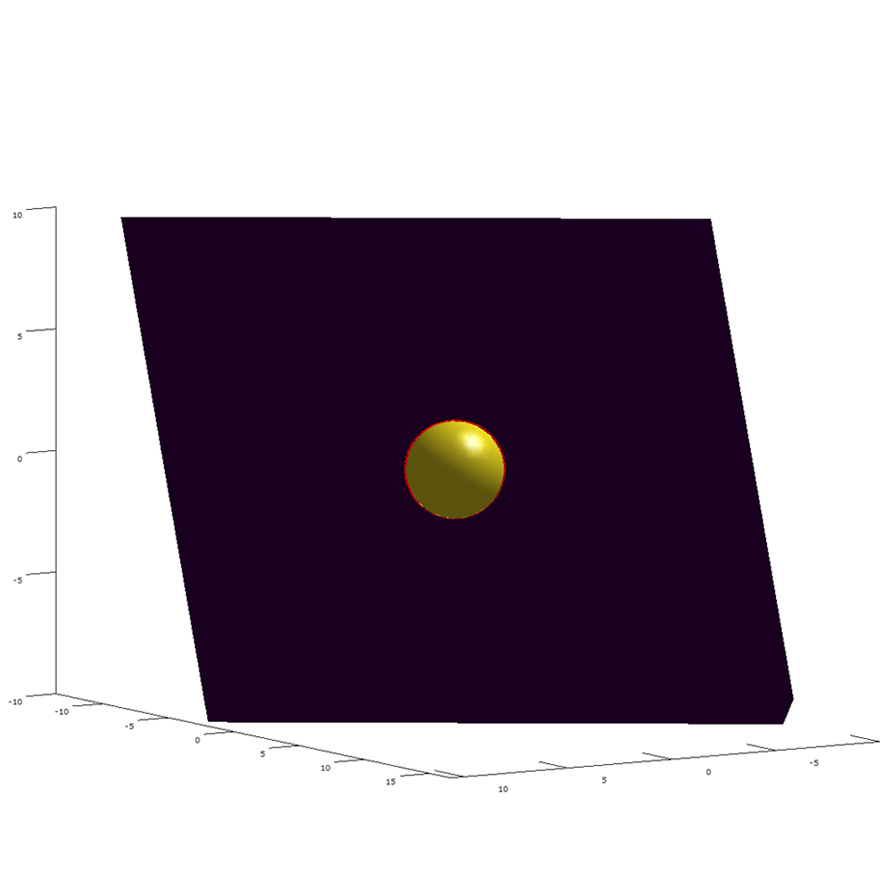
\includegraphics[scale=0.3]{primer1_2}
	\\
	Primer 2:
	\begin{itemize}  
		\item $f_{1}(x,y,z)$ = $x^2 + y^2 + z^2$ = 4
		\item $f_{2}(x,y,z)$ = $x^2 + y^2$ = 1
	\end{itemize}
	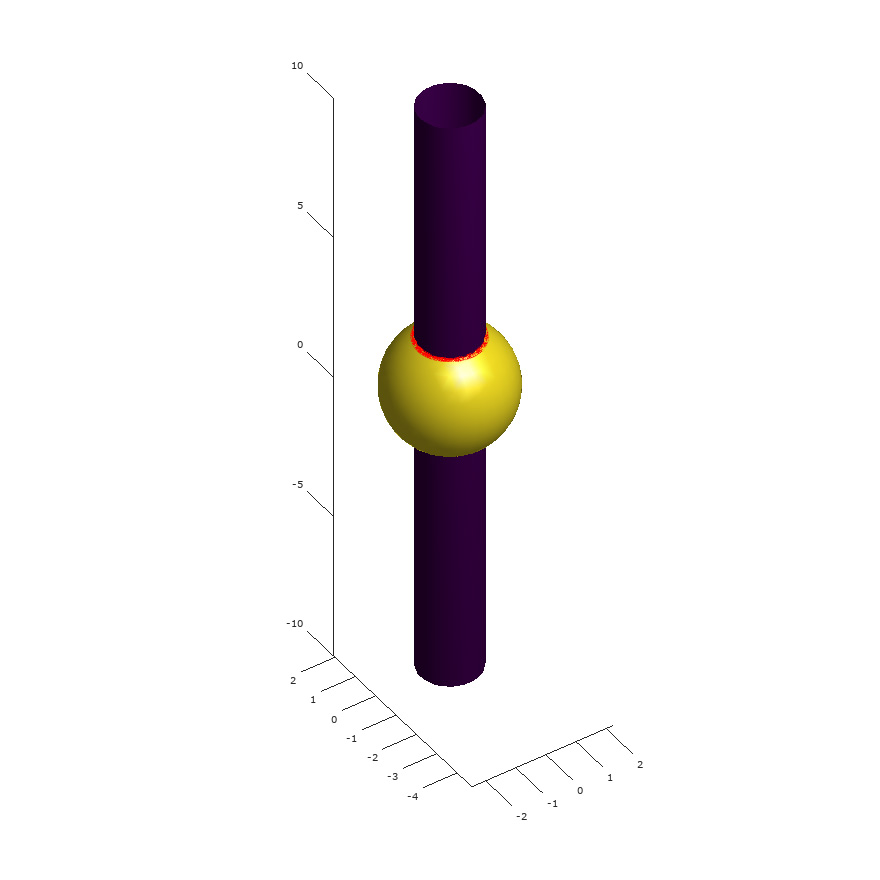
\includegraphics[scale=0.3]{primer2_1}
	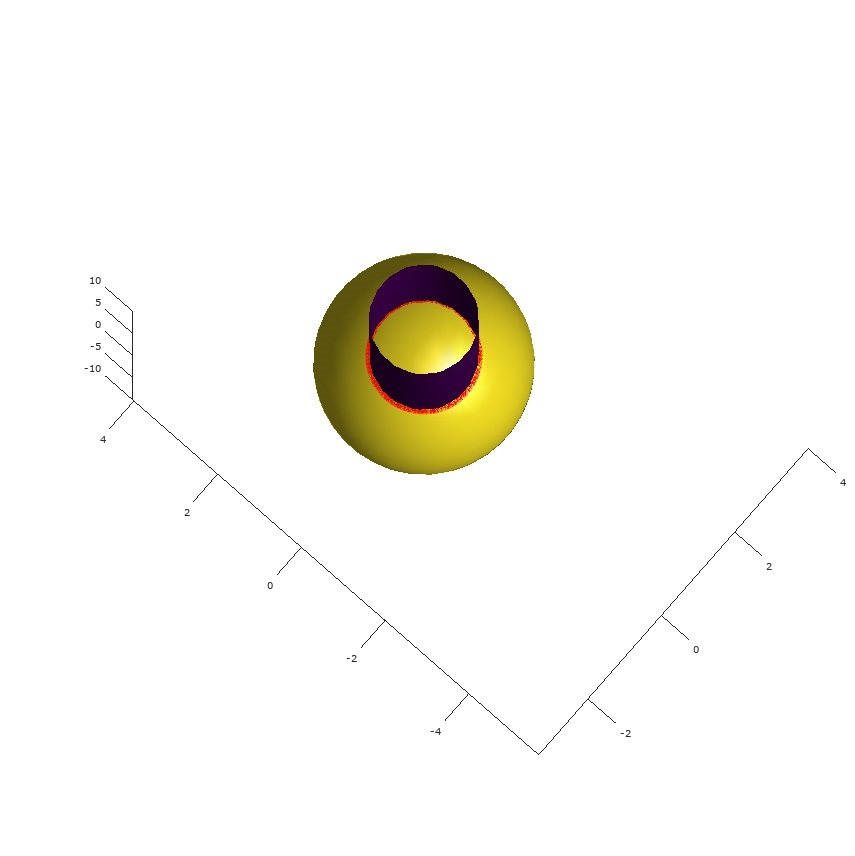
\includegraphics[scale=0.3]{primer2_2}
	\\
	Primer 3:
	\begin{itemize}  
		\item $f_{1}(x,y,z)$ = $x^2 + y^2 + z^2$ = 4
		\item $f_{2}(x,y,z)$ = $y^4 + log(x^2 + 1)z^2 - 4$ = 1
	\end{itemize}
	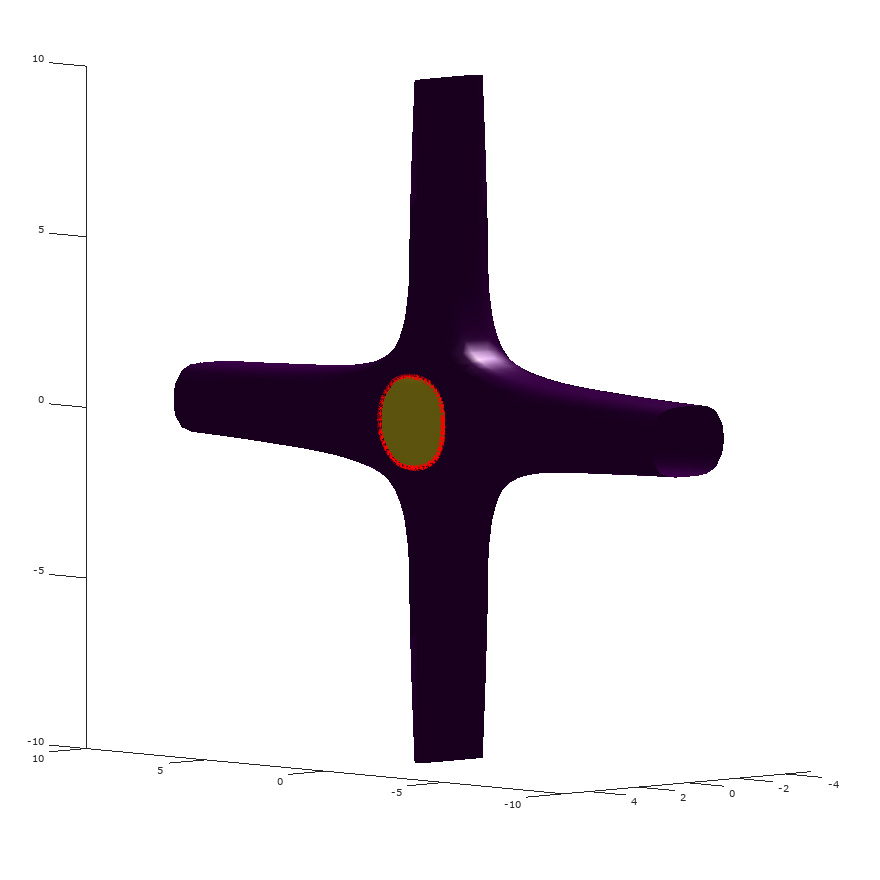
\includegraphics[scale=0.3]{primer3_1}
	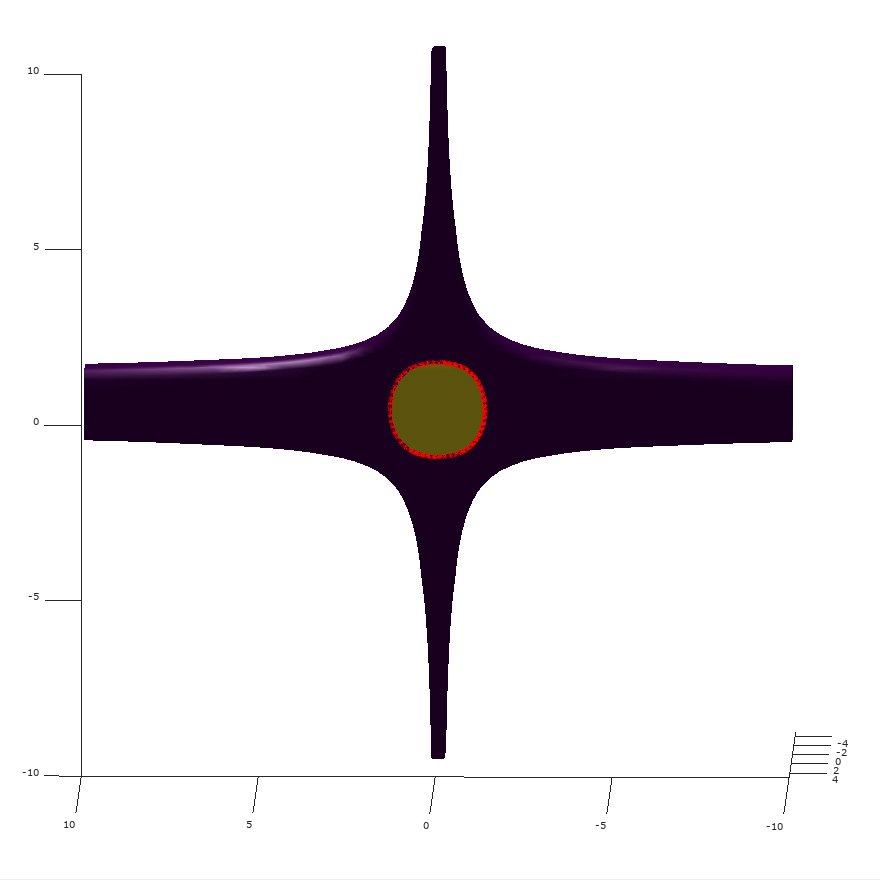
\includegraphics[scale=0.3]{primer3_2}
	\\
	Primer 4:
	\begin{itemize}  
		\item $f_{1}(x,y,z)$ = $x^2 + cos(y)z^2 - 12$ = 4
		\item $f_{2}(x,y,z)$ = $y^4 + log(x^2 + 1)z^2 - 4$ = 1
	\end{itemize}
	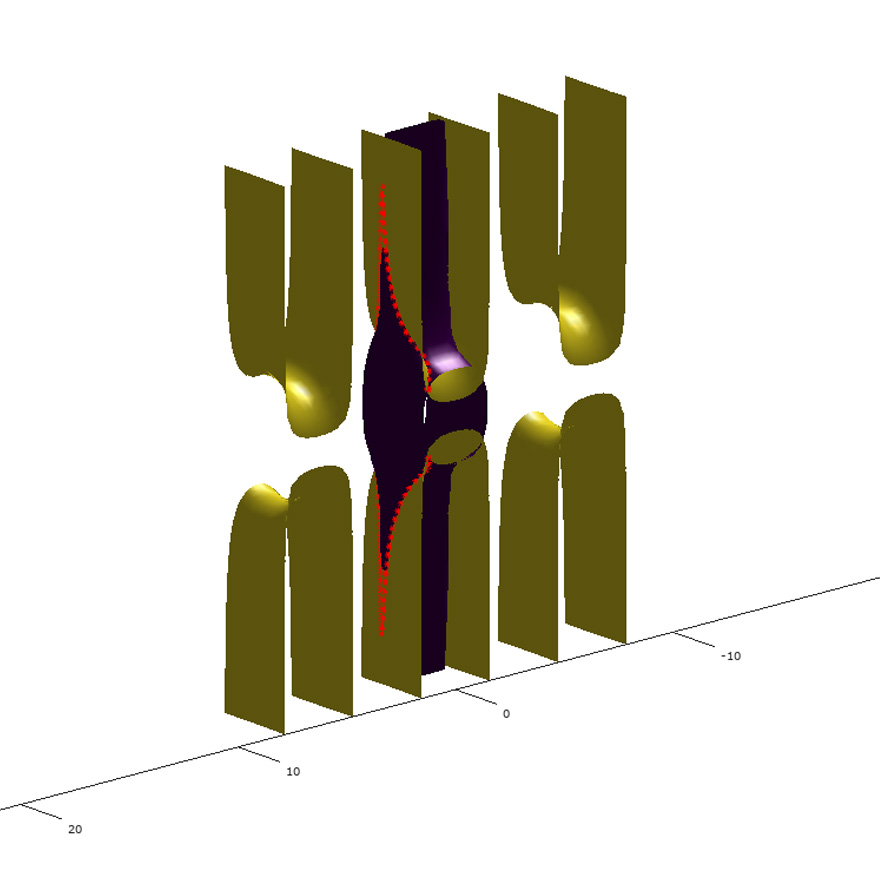
\includegraphics[scale=0.3]{primer4_1}
	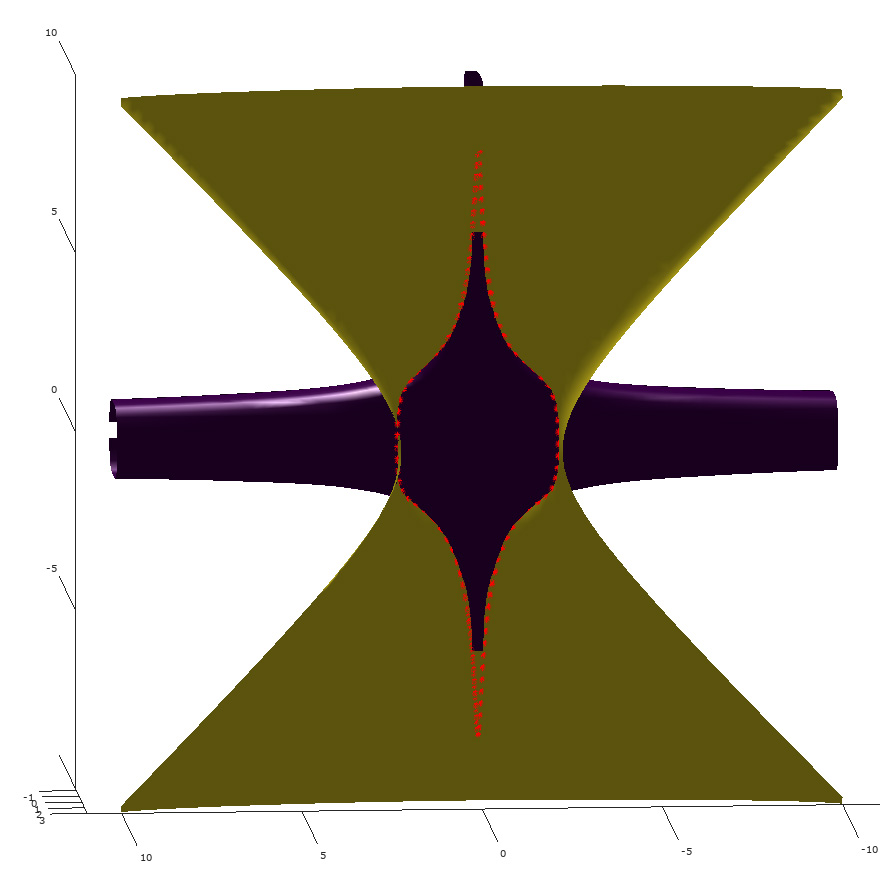
\includegraphics[scale=0.3]{primer4_2}
	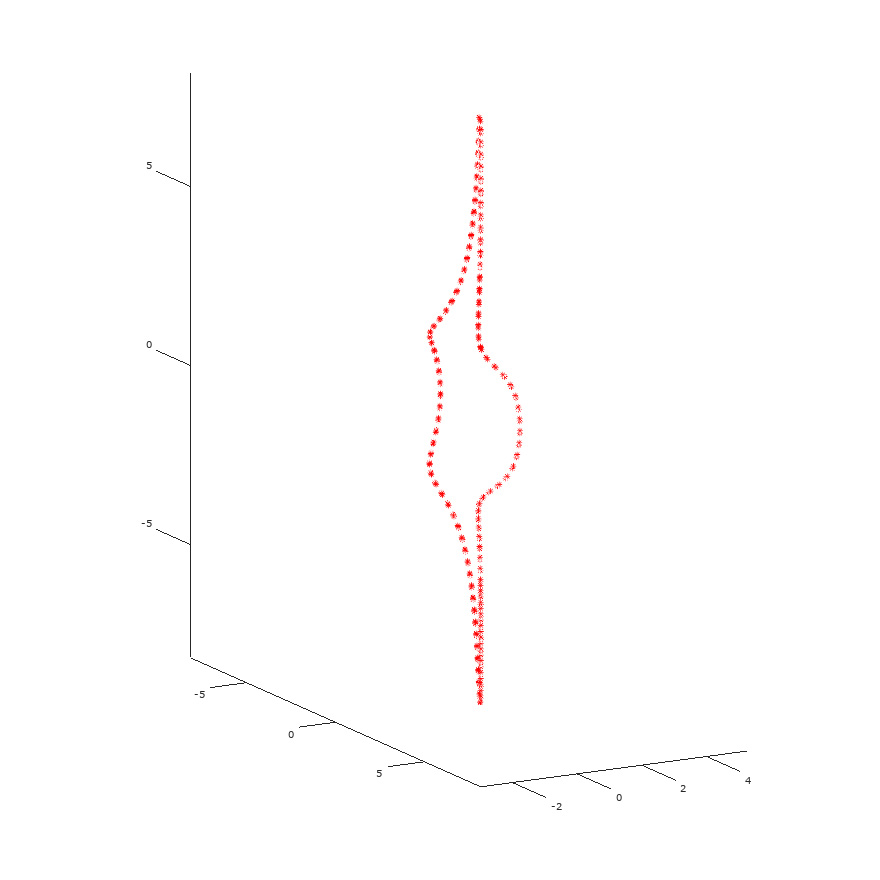
\includegraphics[scale=0.3]{primer4_4}
	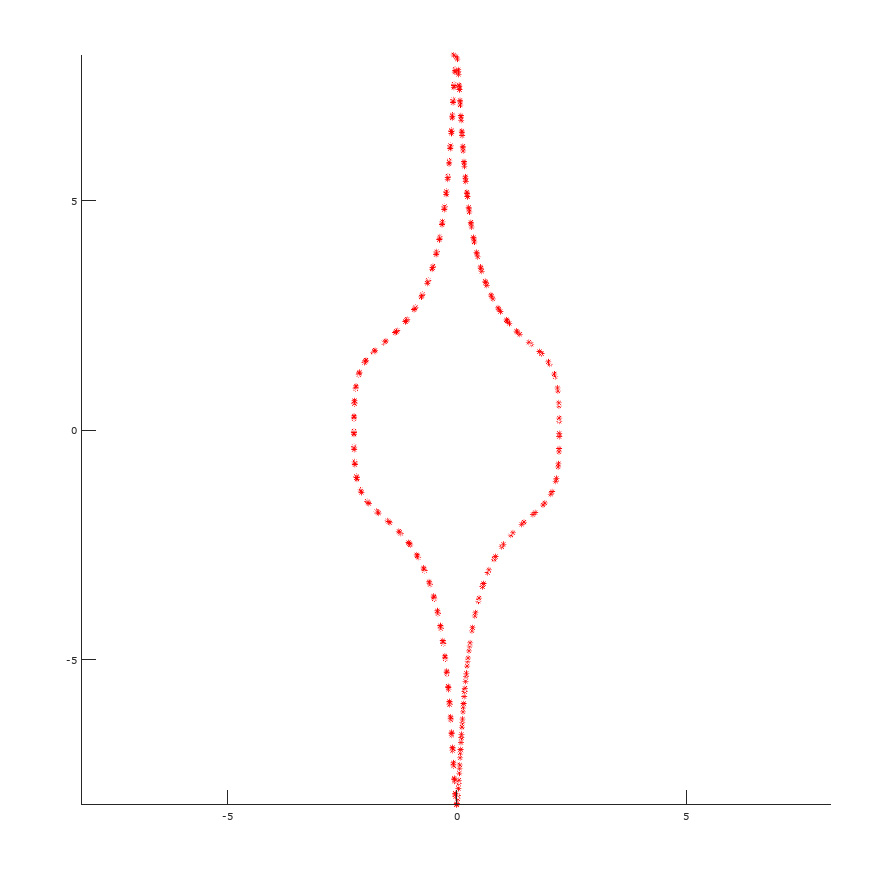
\includegraphics[scale=0.3]{primer4_3}
	\\
	Primer 5:
	\begin{itemize}  
		\item $f_{1}(x,y,z)$ = $e^{(-x^{2}+1)}+y^{2}+z^{2}$ = 3
		\item $f_{2}(x,y,z)$ = $e^{(xyz)}+y^{2}+z^{2}$ = 10
	\end{itemize}
	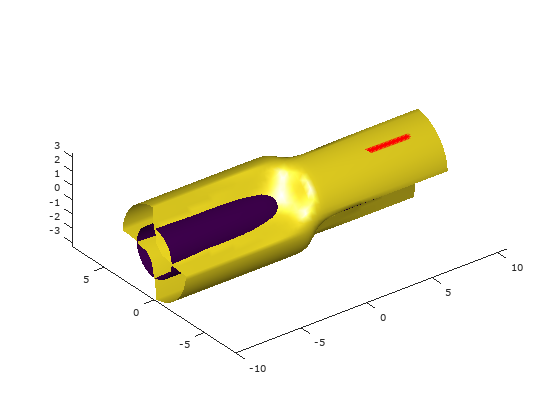
\includegraphics[scale=0.5]{primer5_1}
	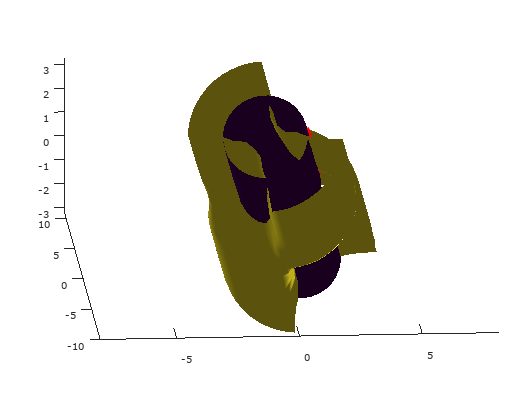
\includegraphics[scale=0.5]{primer5_2} 
	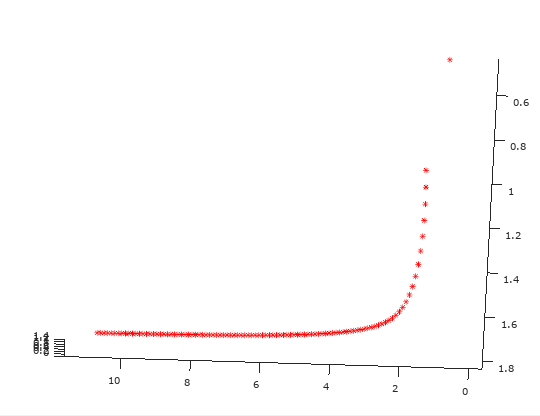
\includegraphics[scale=0.5]{primer5_3}
	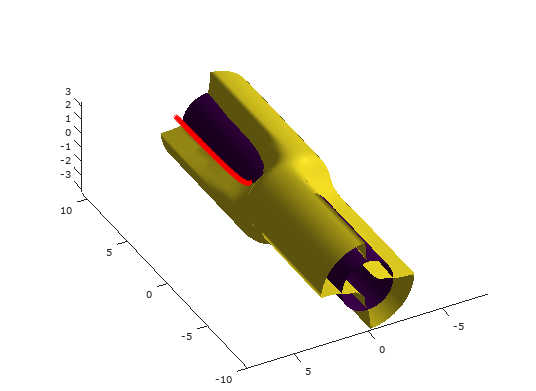
\includegraphics[scale=0.5]{primer5_4} 
	\\
	Primer 6:
	\begin{itemize}  
		\item $f_{1}(x,y,z)$ = $e^{(-x^{2}+1)}+y^{2}+z^{2}$ = 3
		\item $f_{2}(x,y,z)$ = $x^2 + y^2 + z^2$ = 4
	\end{itemize}
	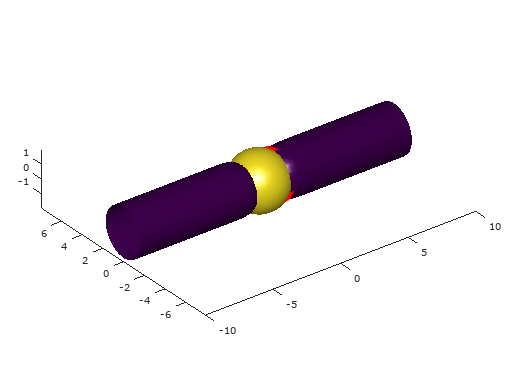
\includegraphics[scale=0.5]{primer6_1}
	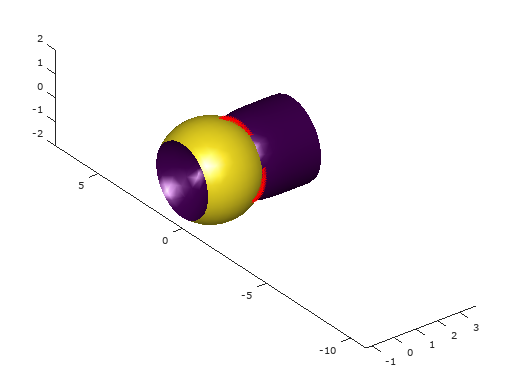
\includegraphics[scale=0.5]{primer6_2}
	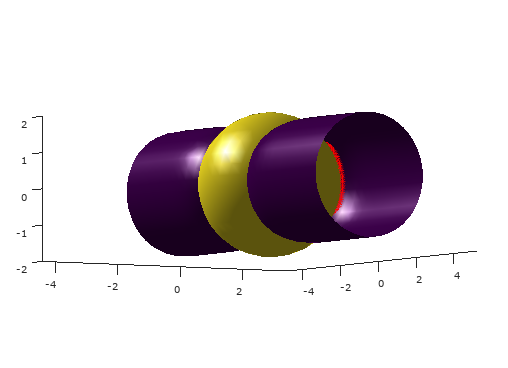
\includegraphics[scale=0.5]{primer6_3}
	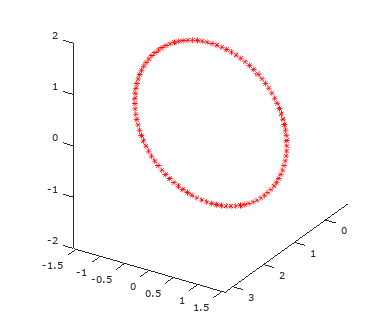
\includegraphics[scale=0.5]{primer6_4} 
	\\
	Primer 7:
	\begin{itemize}  
		\item $f_{1}(x,y,z)$ = $e^{(-x^{2}+1)}+y^{2}+z^{2}$ = 3
		\item $f_{2}(x,y,z)$ =  $x^2 + y^2$ = 1
	\end{itemize}
	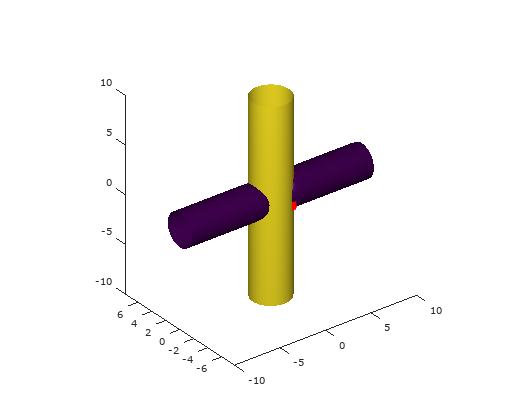
\includegraphics[scale=0.5]{primer7_1}
	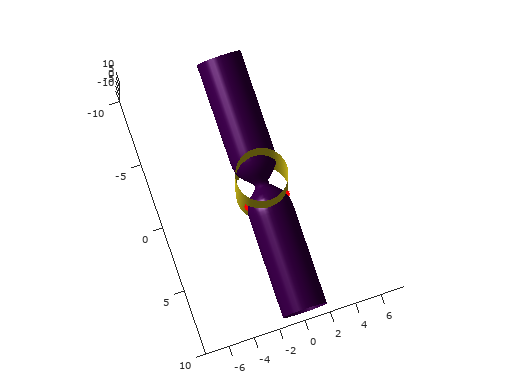
\includegraphics[scale=0.5]{primer7_2}
	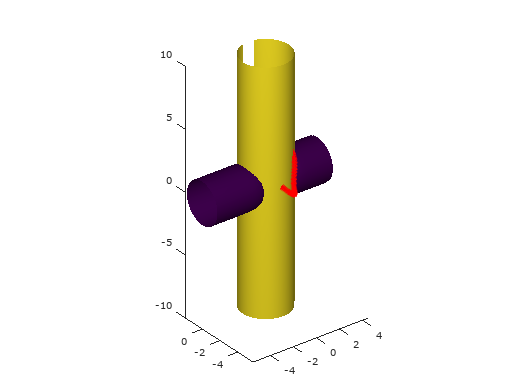
\includegraphics[scale=0.5]{primer7_3}
	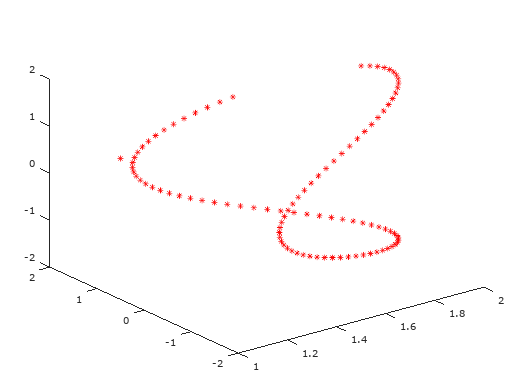
\includegraphics[scale=0.5]{primer7_4} 
	\\
	Primer 8:
	\begin{itemize}  
		\item $f_{2}(x,y,z)$ = $e^{(xyz)}+y^{2}+z^{2}$ = 10
		\item $f_{2}(x,y,z)$ =  $x^2 + y^2$ = 1
	\end{itemize}
	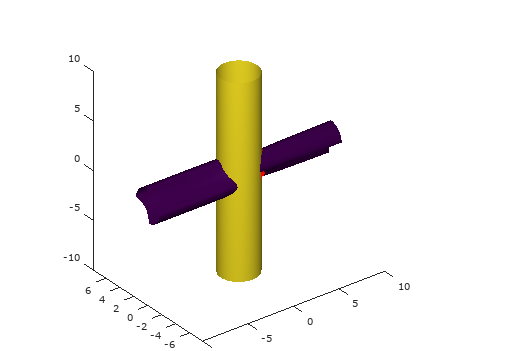
\includegraphics[scale=0.5]{primer8_1}
	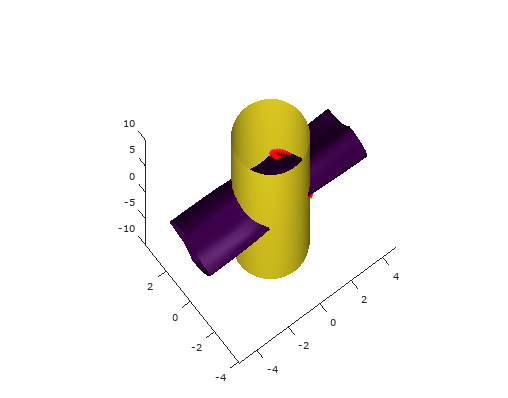
\includegraphics[scale=0.5]{primer8_2}
	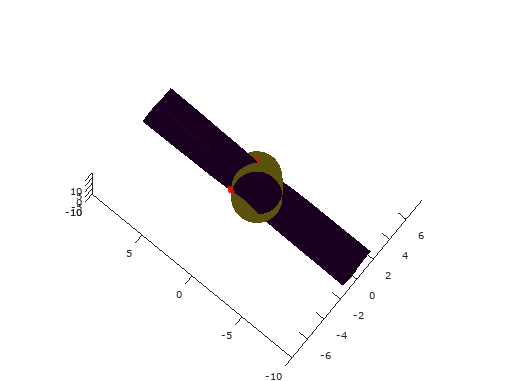
\includegraphics[scale=0.5]{primer8_3}
	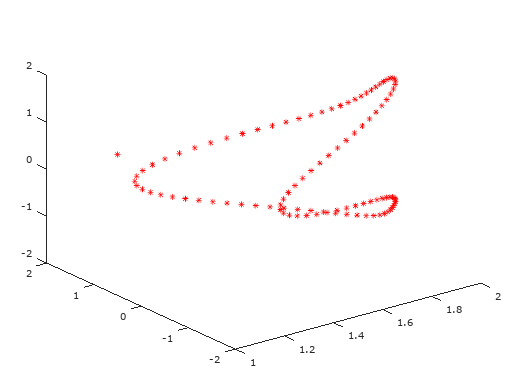
\includegraphics[scale=0.5]{primer8_4} 
	\\	
\section{Analiza povpre\v{c}no \v{s}tevilo korakov Newtonove metode} 
Na konec za vseh osem primerov smo naredili analizo, tako da smo izmerili povpre\v{c}no \v{s}tevilo korakov Newtonove metode z obe metode na dva na\v{c}ina: z adaptivnem in fiksnem koraku. Pri adaptivnem koraku smo izra\v{c}unali tudi minimalno in maksimalno \v{s}tevilo korakov. \\
Primer in rezultati izvajanje enega testa: \\
	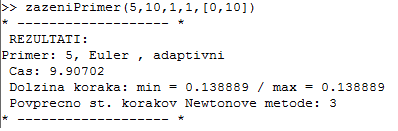
\includegraphics[scale=0.8]{a1}
	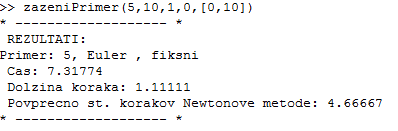
\includegraphics[scale=0.8]{a2}
	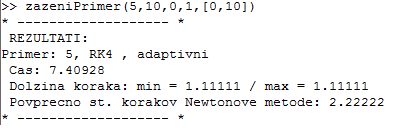
\includegraphics[scale=0.8]{a3}
	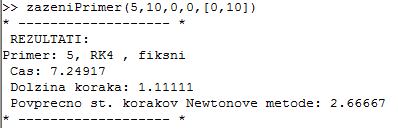
\includegraphics[scale=0.8]{a4} \\ \\
Po izvajanje ta postopek za vseh primerov smo dobili naslenje rezultate: \\
\begin{tabular}{|c | c | c | c | c |} 
 \hline
 \textbf{Funkcije} &\multicolumn{2}{|l|}{\textbf{Euler}} &\multicolumn{2}{|l|}{\textbf{RK4}}\\                
  \small &adaptivno & fiksno & adaptivno & fiksno \\ 
 \hline
 \small{}$f_{1}(x,y,z)=x^{2} + y^{2}+ z^{2}=4$ & & & &\\ 
 \small{}$f_{2}(x,y,z)=x^{2} + y^{2}    =1$  & 3 & 5 & 3 & 3.222 \\
 \hline
 \small{}$f_{1}(x,y,z)=x^{2} + y^{2}+ z^{2}=4$ & & & &\\ 
 \small{}$f_{2}(x,y,z)$ = $3x + 2y + z = 1$  & 3 & 4.222 & 3 & 3.333 \\
 \hline
 \small{}$f_{1}(x,y,z)=x^{2} + y^{2}+ z^{2}=4$ & & & &\\ 
 \small{}$f_{2}(x,y,z)$ = $y^4 + log(x^2 + 1)z^2 - 4 = 1$  & 3 & 5 & 3 & 3.222 \\
 \hline
 \small{}$f_{1}(x,y,z)$ = $x^2 + cos(y)z^2 - 12 = 4$ & & & &\\ 
\small{}$f_{2}(x,y,z)$ = $y^4 + log(x^2 + 1)z^2 - 4 = 1$  & 3 & 4.111 & 2.222 & 2.556 \\
 \hline
 \small{}$f_{1}(x,y,z)$ = $e^{(-x^{2}+1)}+y^{2}+z^{2} = 3$ & & & &\\ 
 \small{}$f_{2}(x,y,z)$ = $e^{(xyz)}+y^{2}+z^{2} = 10$  & 3 & 4.667 & 2.222 & 2.667 \\
 \hline
 \small{}$f_{1}(x,y,z)$ = $e^{(-x^{2}+1)}+y^{2}+z^{2} = 3$ & & & &\\ 
 \small{}$f_{2}(x,y,z)=x^{2} + y^{2}+ z^{2}=4$  & 3 & 5 & 3 & 3.222 \\
 \hline
 \small{}$f_{1}(x,y,z)$ = $e^{(-x^{2}+1)}+y^{2}+z^{2} = 3$ & & & &\\ 
  \small{}$f_{2}(x,y,z)=x^{2} + y^{2}    =1$  & 3 & 5 & 3 & 3.333 \\
  \hline
\small{}$f_{1}(x,y,z)$ = $e^{(xyz)}+y^{2}+z^{2} = 10$ & & & &\\ 
 \small{}$f_{2}(x,y,z)=x^{2} + y^{2}    =1$  & 3 & 5 & 3 & 3.556 \\
  \hline
\end{tabular} \par
Pri bolj kompleksni funkcije kot: $f_{1}(x,y,z)$ = $x^2 + cos(y)z^2 - 12 = 4$  in $f_{2}(x,y,z)$ = $y^4 + log(x^2 + 1)z^2 - 4 = 1$, pri adaptivnem koraku,\v{s}e posebej pri Runge-Kutta metodo smo dobili manj\v{s}e povpre\v{c}no \v{s}tevilo korakov ker je metoda hitro konvergirala; pa tudi minimalno in maksimalno \v{s}tevilo korakov so bili manj\v{s}i kot pri vseh ostalih.\par
Glede na fiksnem koraku spet smo pri\v{s}li do istem zaklju\v{c}ku kot pri adaptivnemu, da bolj kompleksne funkcije hitrej\v{s}e konvergirajo in rabijo manj \v{s}tevilo korakov, ampak \v{s}e vedno ve\v{c} v primerjavi z adaptivnemu. 

\section{Koda}
\begin{lstlisting}[language=Octave]

\end{lstlisting}

\section{Delitev dela v skupini}
\subsection{Programerski del}
\begin{itemize}
	\item 
	\item 
	\item 
	\item  
\end{itemize}
\subsection{Poro\v{c}ilo}
\begin{itemize}
	\item 
	\item 
	\item 
	\item  
\end{itemize}
\section{Reference}
\begin{itemize}
	\item Zapiski s predavanj:diferencialne ena\v{c}be
\end{itemize}
\end{document}
